\documentclass[../HAFiscal]{subfiles}
\begin{document}

\section{Linearity of the check stimulus}
\label{app:CheckMultiplier}

Table \ref{multipliers_checklinearity} shows the amount of additional consumption stimulated (as \% of baseline consumption) caused by stimulus checks of different sizes as well as their net-present value multiplier. The table shows that the impact of the check stimulus experiment scales roughly linearly with the size of the stimulus check, leaving the multiplier largely unaffected by the size of check.

\begin{table}[h] 
	\center
	\input Code/HA-Models/FromPandemicCode/Tables/Multiplier_DifferentCheckSizes.tex
	\caption{Multipliers for different sizes of the stimulus check}
	\label{multipliers_checklinearity}
\end{table}

\section{Estimating discount factor distributions for different interest rates}
\label{app:DF_R}

Figure~\ref{fig:LorenzPts_robustness_R} shows the fit of the liquid wealth distribution for interest rates of $0.5$ percent and $1.5$ percent per quarter. In both cases, the estimation exactly matches the median liquid wealth to permanent income ratios for each education group listed in Panel~B of Table~\ref{tab:estimBetas}. 

%\begin{table}{th}
%\begin{center}
%\begin{tabular}{lccc}
%	\multicolumn{4}{l}{Panel (B) Estimation targets} \\ \midrule
%	& Dropout & Highschool & College \\ \midrule
%	Median LW/PI (data) & 4.64 & 30.2 & 112.8 \\ 
%	Median LW/PI (model, $R = 1.005$) & 4.64 & 30.2 & 112.8 \\	
%	Median LW/PI (model, $R = 1.01$) & 4.64 & 30.2 & 112.8 \\
%	Median LW/PI (model, $R = 1.015$) & 4.64 & 30.2 & 112.8 \\ \bottomrule
%\end{tabular} \\ \\ 
%\end{center}	
%\end{table}

\begin{figure}[th]
	\begin{center}
		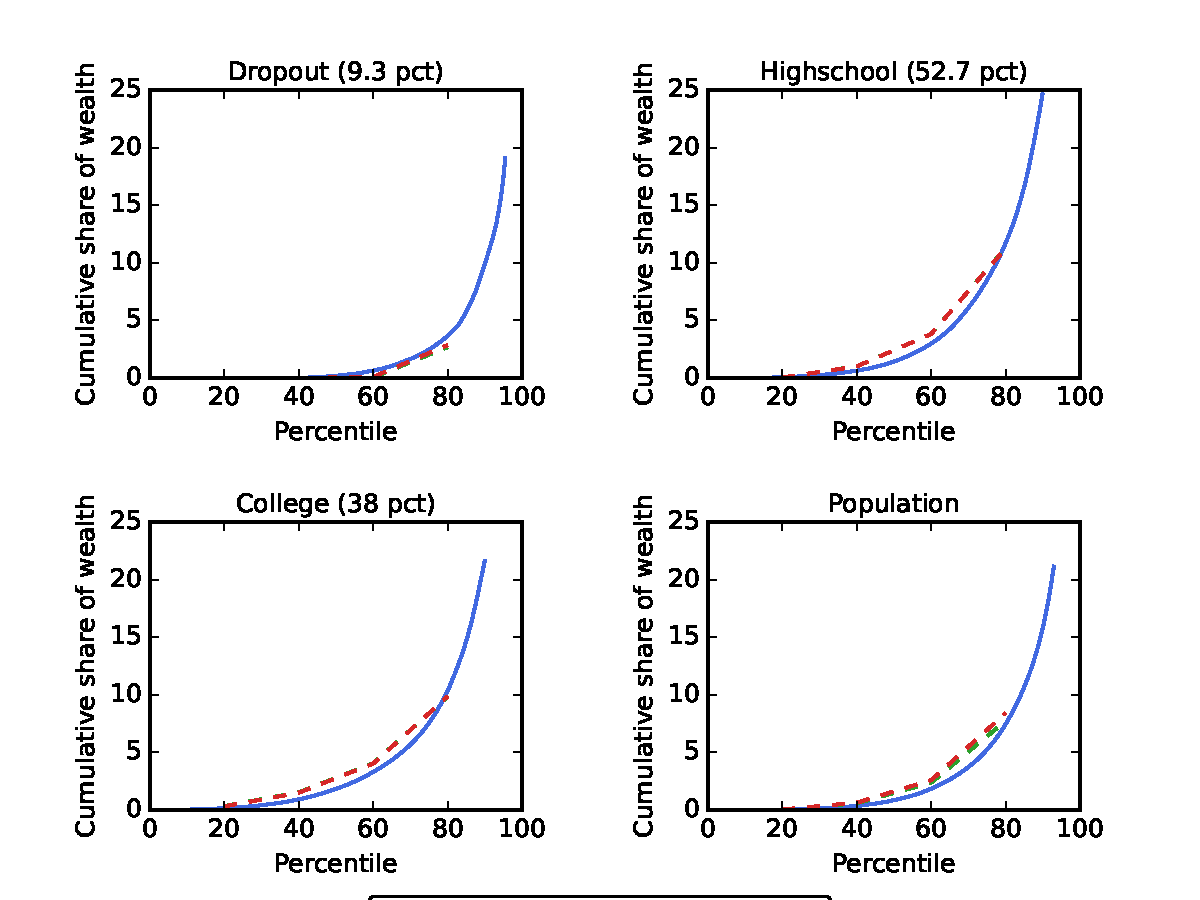
\includegraphics[width=.9\textwidth]{../Figures/LorenzPoints_robustness_R.pdf}
		\caption{Distributions of liquid wealth within each educational group and for the whole population from the 2004 Survey of Consumer Finance and from the estimated model for different values of the interest rate, $R$.}
		\label{fig:LorenzPts_robustness_R}
	\end{center}
\end{figure}

\end{document}	
